% =============================================================================
%  Irreducible Multi-Scale Governance: Composition and Limits of
%  Atomic Admission Systems
%  Paper 4 of 6 — Agent Governance Series
% =============================================================================
\documentclass[11pt]{article}

% --- Encoding & fonts (matches ACP) ---
\usepackage[utf8]{inputenc}
\usepackage[T1]{fontenc}
\usepackage{lmodern}
\usepackage[protrusion=true,expansion=false]{microtype}
\setlength{\emergencystretch}{3em}

% --- Page geometry ---
\usepackage[margin=1in, top=1.1in, bottom=1.1in]{geometry}

% --- Math ---
\usepackage{amsmath,amssymb,amsthm}

% --- Tables & figures ---
\usepackage{booktabs}
\usepackage{graphicx}
\usepackage{caption}
\captionsetup{font=small,labelfont=bf}

% --- Hyperlinks (matches ACP: colorlinks, no boxes) ---
\usepackage[colorlinks=true,
            linkcolor=blue!70!black,
            citecolor=blue!70!black,
            urlcolor=blue!70!black]{hyperref}

% --- Misc ---
\usepackage{xcolor}
\usepackage{enumitem}
\usepackage[numbers,sort&compress]{natbib}
\usepackage{tikz}
\usetikzlibrary{shapes.geometric,arrows.meta,positioning,fit,backgrounds}
\usepackage{pgfplots}
\pgfplotsset{compat=1.18}
\usepackage{array}
\usepackage{multirow}

% --- Section formatting (matches ACP) ---
\usepackage{titlesec}
\titleformat{\section}{\large\bfseries}{\thesection}{1em}{}
\titleformat{\subsection}{\normalsize\bfseries}{\thesubsection}{1em}{}

% --- Paragraph spacing (matches ACP) ---
\setlength{\parskip}{0.5em}
\setlength{\parindent}{0pt}

% ---------------------------------------------------------------------------
%  Theorem environments
% ---------------------------------------------------------------------------
\newtheorem{theorem}{Theorem}[section]
\newtheorem{lemma}[theorem]{Lemma}
\newtheorem{corollary}[theorem]{Corollary}
\newtheorem{proposition}[theorem]{Proposition}
\newtheorem{definition}[theorem]{Definition}
\newtheorem{assumption}[theorem]{Assumption}
\newtheorem{example}[theorem]{Example}
\newtheorem{remark}[theorem]{Remark}
\newtheorem{observation}[theorem]{Observation}

% ---------------------------------------------------------------------------
%  Macros
% ---------------------------------------------------------------------------
\newcommand{\Agents}{\mathcal{A}}
\newcommand{\Dec}{\mathcal{D}}
\newcommand{\Dhat}{\widehat{D}}
\newcommand{\Azero}{\mathcal{A}_0}
\newcommand{\allow}{\texttt{Allow}}
\newcommand{\deny}{\texttt{Deny}}
\newcommand{\escalate}{\texttt{Escalate}}
\newcommand{\Layer}[1]{L_{#1}}
\newcommand{\State}[1]{S_{#1}}
\newcommand{\Trans}[1]{\delta_{#1}}
\newcommand{\Sum}[1]{\lambda_{#1}}
\newcommand{\Comp}{\otimes_\kappa}
\newcommand{\AsyncComp}{\xrightarrow{\kappa}}
\newcommand{\join}{\sqcup}

% ---------------------------------------------------------------------------
\begin{document}

\title{\textbf{Irreducible Multi-Scale Governance: Composition and\\
Limits of Atomic Admission Systems}}

\author{Marcelo Fernandez \\
TraslaIA \\
\texttt{info@traslaia.com}}

\date{2026}
\maketitle

% ---------------------------------------------------------------------------
\begin{abstract}
We formalize the compositional structure of a four-layer agent governance
architecture comprising an atomic decision boundary~\cite{fernandez2026a},
a stateful enforcement protocol~\cite{fernandez2026b}, a behavioral invariant
monitor~\cite{fernandez2026c}, and a fair access allocator~\cite{fairgov26}.
We introduce a multi-scale composition model that distinguishes synchronous
coupling at the request level from asynchronous coupling at the trace and
population level. We prove three results: (1)~\emph{Interface Compatibility}
--- the composed system preserves the guarantees of all layers at their
respective operating scales; (2)~\emph{Feedback Convergence} --- the
closed-loop system induced by thresholded feedback from the monitoring layer
to the enforcement layer converges to a bounded deviation region under
regularity conditions; (3)~\emph{Irreducibility under Finite Observability}
--- under finite observability (finite state spaces, bounded inter-layer
summaries, local decision-making) and summary-based inter-layer interfaces,
no composition of fewer than four layers can simultaneously guarantee
strong atomicity, bounded non-identifiability of behavioral contracts, exact
fairness at the actor level, and Sybil robustness.
This irreducibility result establishes that the
four-layer architecture is structurally necessary within this observability
model, not an artifact of design
choices. The four layers correspond to four orthogonal projections of the
governance space --- temporal (atomicity), state (enforcement history),
behavioral (drift monitoring), and population (fair allocation) --- and
the irreducibility result shows that no single mechanism can cover two
projections simultaneously under finite observability.
We validate the three theorems with a controlled ablation study
($8 \times 4 \times 5 = 160$ trials), a feedback convergence experiment
(10 seeds, 1000 steps each), and an interface compatibility check (20 trials),
using the real ACP risk engine and IML deviation estimator.
This paper is Paper~4 of the 6-paper Agent Governance Series:
atomic boundaries (P0,~\cite{fernandez2026a}),
stateful enforcement---ACP (P1,~\cite{fernandez2026b}),
behavioral drift---IML (P2,~\cite{fernandez2026c}),
fair allocation (P3,~\cite{fairgov26}),
and runtime execution validity---RAM (P5,~\cite{fernandez2026ram}).
Paper~4 proves the four-layer architecture (L0--L3) is irreducible;
Paper~5 provides the operational closure for L2 at runtime.
\end{abstract}

\tableofcontents
\newpage

% ===========================================================================
\section{Introduction}
\label{sec:intro}
% ===========================================================================

Consider an autonomous agent authorized to execute financial transactions on
behalf of a user. A na\"{i}ve admission policy checks each request individually:
does the agent hold a valid capability token? Is the request within the
authorized amount? These per-request checks are necessary but not sufficient.
An adversarial agent can submit a sequence of individually valid requests---each
below the detection threshold---that collectively constitute a behavioral
anomaly: systematically draining accounts, probing rate limits, or accumulating
influence beyond any single transaction's scope. Per-request enforcement,
however sophisticated, cannot see this pattern without trace-level observation.

Now add trace-level monitoring. The monitor detects the drift pattern and
signals an anomaly. But the signal must act on \emph{something}: it must alter
admission policy, or reallocate access, or both. If no enforcement layer
receives and acts on the signal, the monitor is observational but not
corrective. And even a system that enforces + monitors may still be
manipulated at the population level: an adversary who controls multiple
identities can distribute their requests across agents, defeating per-agent
history and making drift appear as legitimate population variance rather than
concentrated abuse. Addressing this requires a fourth mechanism, one that
tracks population-level allocation and detects concentration across identities.

This paper asks and answers the structural question: \emph{how many
layers does a sound governance architecture require, and why?} We prove that
four is not a design choice but a structural necessity under the constraint
of finite-state, local-observability systems. The result---
Theorem~\ref{thm:irreducibility}, \emph{Irreducibility under Finite
Observability}---shows that no composition of fewer than four layers can
simultaneously guarantee strong atomicity, behavioral non-identifiability
bounds, exact actor-level fairness, and Sybil robustness. The four layers
are four irreducible projections of the governance space, not four
implementations of the same concept.

We formalize each layer as a transducer $\Layer{i} = (\State{i}, \Sigma_i,
\Trans{i}, \Sum{i})$ and define two composition regimes: synchronous
composition $\Comp$ for the per-request layers (Papers~0 and~1), and
asynchronous coupling $\AsyncComp$ for the trace-window and epoch-level
layers (Papers~2 and~3). This multi-scale distinction is the key technical
contribution of the model: forcing all layers into a single temporal regime
produces a formally incorrect semantics. Three main theorems are proved:
Interface Compatibility (Theorem~\ref{thm:compatibility}), Feedback
Convergence (Theorem~\ref{thm:convergence}), and Irreducibility
(Theorem~\ref{thm:irreducibility}).

\paragraph{Position in the series.}
The paper synthesizes and extends:
\begin{itemize}[noitemsep]
  \item \textbf{Paper~0}~\cite{fernandez2026a}: Atomic Decision Boundaries ---
    LTS model $M = (S, \mathit{Act}, \to)$; decision function
    $F: S \times \mathit{Act} \to \Dec \times \hat{S}$; proof that split
    systems cannot guarantee atomicity (Theorem~5.1); Corollary~5.6.
  \item \textbf{Paper~1}~\cite{fernandez2026b}: Agent Control Protocol (ACP)
    --- evaluate-then-mutate pipeline; BAR-Monitor; Capability Token; Audit
    Ledger; TLA+ verified; refines $F$ under TA1 (serializable ledger) and
    TA2 (atomic commit).
  \item \textbf{Paper~2}~\cite{fernandez2026c}: From Admission to Invariants
    (IML) --- Non-Identifiability Theorem: $\Azero \notin \sigma(g)$;
    $\Dhat = 0.40 D_t + 0.35 D_c + 0.25 D_l$; detection delay $T^*(\theta)$;
    Assumption~A3 ($K$-Lipschitz regularity).
  \item \textbf{Paper~3}~\cite{fairgov26}: Fair Atomic Governance ---
    allocation mechanisms M1/M2/M3; Sybil Amplification (Thm~5.1);
    Strategy-Proofness Impossibility (Thm~5.4); BAR-Monitor interference.
\end{itemize}

\paragraph{Outline.}
Section~\ref{sec:prelim} reviews the four layers and their key results.
Section~\ref{sec:model} defines the formal composition model.
Section~\ref{sec:thm1} proves Interface Compatibility.
Section~\ref{sec:thm2} proves Feedback Convergence.
Section~\ref{sec:thm3} proves Irreducibility.
Section~\ref{sec:empirical} gives the cross-layer empirical analysis.
Section~\ref{sec:discussion} discusses implications.
Section~\ref{sec:conclusion} concludes.

% ===========================================================================
\section{Preliminaries}
\label{sec:prelim}
% ===========================================================================

This section summarizes the formal results from Papers~0--3 that are
directly used in the composition model and theorems. Readers familiar with
the series may skip to Section~\ref{sec:model}.

\subsection{Paper~0: Atomic Decision Boundaries~\cite{fernandez2026a}}

A \emph{governance system} is modeled as a labeled transition system (LTS)
$M = (S, \mathit{Act}, \to)$, where $S$ is a state space, $\mathit{Act}$ is
an action alphabet, and ${\to} \subseteq S \times \mathit{Act} \times S$ is
a transition relation. An \emph{atomic decision boundary} is a function
\[
  F: S \times \mathit{Act} \to \Dec \times \hat{S}, \quad
  \Dec = \{\allow, \escalate, \deny\},
\]
such that evaluation of $F(s, a)$ and the resulting state transition
$s \to s'$ occur as a single indivisible step. The central theorem of
Paper~0 (Theorem~5.1) proves that \emph{split systems}---in which evaluation
and mutation occur in separable steps that may interleave under concurrency---
cannot guarantee that the committed state matches the decision computed at
evaluation time. This formalizes TOCTOU as a structural impossibility, not
an implementation artifact.

\subsection{Paper~1: Agent Control Protocol~\cite{fernandez2026b}}

ACP is a stateful admission control protocol that \emph{refines} $F$ under
two transactional assumptions:
\begin{itemize}[noitemsep]
  \item \textbf{TA1} (Serializable ledger): the per-agent Audit Ledger
    supports serializable transactions.
  \item \textbf{TA2} (Atomic commit): the evaluate-then-mutate pipeline
    commits the decision and state update as a single atomic transaction.
\end{itemize}
{\sloppy
ACP maps the abstract state $s \in S$ to a concrete tuple
$(ledger, riskScore, cooldown, agentState)$, and the decision function $F$ to
the evaluate-then-mutate pipeline. Per-agent behavioral history is maintained
across requests via the Capability Token and Audit Ledger. The BAR (Boundary
Activation Rate) monitor tracks the ratio of non-trivially-enforced decisions
and serves as an early warning signal for behavioral drift. The protocol is
TLA$^+$ verified, with three invariants confirmed over $4.29 \times 10^9$ states.
\par}

\subsection{Paper~2: From Admission to Invariants~\cite{fernandez2026c}}

The IML framework addresses the observability gap above the enforcement layer.
Let $\tau = (a_1, \ldots, a_T)$ be an agent trace and
$g: \Sigma^* \to \{0,1\}$ the \emph{enforcement projection} mapping traces to
enforcement signals. The key result is the \textbf{Non-Identifiability Theorem}
(Theorem~3.2 of Paper~2):
\[
  \Azero \notin \sigma(g),
\]
where $\Azero \subseteq \Sigma^*$ is the admissible behavior contract and
$\sigma(g)$ is the $\sigma$-algebra generated by $g$. In plain terms: no
function of the enforcement decisions alone can determine whether an agent's
behavior contract has been violated. This is an information-theoretic limit,
not a limitation of any specific enforcement mechanism.

The IML deviation estimator is defined as:
\[
  \Dhat_t = 0.40\, D_t + 0.35\, D_c + 0.25\, D_l \;\in [0,1],
\]
where $D_t$ captures temporal irregularity, $D_c$ capability diversity, and
$D_l$ latency deviation. The detection delay $T^*(\theta)$ is the minimum
window length required to detect sustained drift at significance level
$\theta$. Assumption~A3 of Paper~2 requires that $\Dhat_t$ is $K$-Lipschitz
in the underlying behavioral parameters, ensuring smoothness of the
feedback signal.

\subsection{Paper~3: Fair Atomic Governance~\cite{fairgov26}}

Paper~3 studies the fairness of access to the governance boundary. Four
allocation mechanisms are analyzed:
\begin{itemize}[noitemsep]
  \item \textbf{M1} (Per-Agent Token Bucket): fixed token budget per agent.
  \item \textbf{M2} (Round-Robin Fair Queuing): admission in round-robin order across agents.
  \item \textbf{M3} (Actor-Aware Rate Limiting): per-actor rate control preventing Sybil amplification.
  \item \textbf{M4} (Weighted Fair Queuing): admission weighted by actor share $1/m_j$.
\end{itemize}
Key impossibility results include:
\begin{itemize}[noitemsep]
  \item \textbf{Sybil Amplification} (Thm~5.1): under any identity-oblivious
    mechanism (M1, M2), an adversary controlling $k$ identities can amplify resource
    consumption by a factor proportional to $k$.
  \item \textbf{Strategy-Proofness Impossibility} (Thm~5.4): no mechanism
    simultaneously achieves efficiency, fairness at the actor level, and
    Sybil robustness under population heterogeneity; achieving both requires
    actor-aware state aggregation (M3/M4).
  \item \textbf{BAR-Monitor Interference}: under identity-oblivious mechanisms
    (M1/M2), Sybil attacks depress the BAR signal, masking enforcement
    degradation from the IML monitor.
\end{itemize}
The agent population is denoted $\Agents$ (macro \verb|\Agents| = $\mathcal{A}$),
with allocation vectors $\alpha \in \Delta(\Agents)$ denoting probability
distributions over agents.

\subsection{Notation Summary}

Table~\ref{tab:notation} collects the notation unified across the series.

\begin{table}[ht]
\centering\small
\caption{Unified notation for the Agent Governance Series.}
\label{tab:notation}
\begin{tabular}{lp{5.8cm}l}
\toprule
\textbf{Symbol} & \textbf{Meaning} & \textbf{Source} \\
\midrule
$\Dec = \{\allow,\escalate,\deny\}$ & Decision domain$^{\dagger}$ & Papers~0--4 \\
$\join$ & Join: severity order $\allow \prec \escalate \prec \deny$ & Papers~0--4 \\
$F: S \times \mathit{Act} \to \Dec \times \hat{S}$ & Atomic decision function & Paper~0 \\
$g: \Sigma^* \to \{0,1\}$ & Enforcement projection & Paper~2 \\
$\Azero \subseteq \Sigma^*$ & Admissible behavior contract & Paper~2 \\
$\Dhat_t \in [0,1]$ & IML deviation estimate & Paper~2 \\
$\Agents$ ($= \mathcal{A}$) & Agent population & Paper~3 \\
$\alpha_t \in \Delta(\Agents)$ & Allocation distribution & Paper~3 \\
$L_i = (S_i, \Sigma_i, \delta_i, \lambda_i)$ & Governance layer & Paper~4 \\
$\otimes_\kappa$ & Synchronous composition & Paper~4 \\
$\xrightarrow{\kappa}$ & Asynchronous coupling & Paper~4 \\
\bottomrule
\end{tabular}
\smallskip

\noindent\small $^{\dagger}$\,Papers~0 and~3 write $\textsc{Refuse}$ for the
non-admissible outcome; this paper writes $\deny$ as a synonym, following
ACP's \texttt{DENIED} response (Paper~1).  The decision domain
$\Dec = \{\allow,\escalate,\deny\}$ is the same object across all papers.
\end{table}

% ===========================================================================
\section{Multi-Scale Composition Model}
\label{sec:model}
% ===========================================================================

\subsection{Layer Definition}

\begin{definition}[Layer]
\label{def:layer}
A \emph{governance layer} is a tuple
\[
  \Layer{i} = (\State{i},\, \Sigma_i,\, \Trans{i},\, \Sum{i}),
\]
where $\State{i}$ is a finite internal state space, $\Sigma_i$ is an input
alphabet, $\Trans{i}: \State{i} \times \Sigma_i \to \State{i} \times M_i
\times \Dec$ is the transition function producing a new state, a message
$m \in M_i$, and a local decision $d \in \Dec$, and
$\Sum{i}: \State{i} \to \Lambda_i$ is the \emph{observable summary} function
projecting internal state to a bounded summary space $\Lambda_i$.
\end{definition}

The decision space $\Dec = \{\allow, \escalate, \deny\}$ is equipped with a
partial order $\allow \prec \escalate \prec \deny$. The join $\join$ denotes
the least upper bound under this order: $d \join d' = \max_\prec(d, d')$.

\subsection{The Four Layers of the Series}

The four layers operate at distinct temporal scales:

\begin{itemize}[noitemsep]
  \item $\Layer{0}$: Atomic boundary layer from Paper~0~\cite{fernandez2026a}.
    Operates \emph{per request}. Enforces the atomicity condition: the decision
    function $F: S \times \mathit{Act} \to \Dec \times \hat{S}$ produces
    a decision and state transition as a single atomic step.
  \item $\Layer{1}$: ACP enforcement layer from
    Paper~1~\cite{fernandez2026b}. Operates \emph{per request}. Maintains
    per-agent state (Capability Token, Audit Ledger), enforces evaluate-then-mutate
    pipeline under TA1 and TA2.
  \item $\Layer{2}$: IML behavioral monitor from
    Paper~2~\cite{fernandez2026c}. Operates \emph{per trace window} $W_t$ of
    $n$ consecutive requests. Produces deviation estimate
    $\Dhat_t = 0.40 D_t + 0.35 D_c + 0.25 D_l \in [0,1]$.
  \item $\Layer{3}$: Fair allocator from
    Paper~3~\cite{fairgov26}. Operates \emph{per epoch} $E_t$
    (multiple windows). Receives $\Dhat_t$ and produces allocation
    $\alpha_t \in \Delta(\Agents)$ over the agent population $\Agents$.
\end{itemize}

\subsection{Synchronous Composition}

$\Layer{0}$ and $\Layer{1}$ couple synchronously because both must act on
every request.

\begin{definition}[Synchronous composition]
\label{def:sync}
The \emph{synchronous composition} $\Layer{0} \Comp \Layer{1}$ is the tuple
\[
  (\State{0} \times \State{1},\; \Sigma,\; \Trans{\otimes},\; \Sum{\otimes}),
\]
where the per-step dynamics are:
\begin{align*}
  (s_0', m_0, d_0) &= \Trans{0}(s_0, x), \\
  x_1 &= \kappa(m_0), \\
  (s_1', m_1, d_1) &= \Trans{1}(s_1, x_1), \\
  d_\otimes &= d_0 \join d_1,
\end{align*}
for input $x \in \Sigma$, coupling function
$\kappa: M_0 \to \Sigma_1$, and joint summary
$\Sum{\otimes}(s_0, s_1) = (\Sum{0}(s_0), \Sum{1}(s_1))$.
\end{definition}

The join $d_\otimes = d_0 \join d_1$ ensures the composed system is at least
as restrictive as the more restrictive of the two layers.

\subsection{Asynchronous Coupling}

$\Layer{1}$, $\Layer{2}$, and $\Layer{3}$ couple asynchronously, operating
at different temporal scales.

\begin{definition}[Asynchronous coupling chain]
\label{def:async}
The \emph{asynchronous coupling chain}
$\Layer{1} \AsyncComp^{W_t}_\kappa \Layer{2} \AsyncComp^{E_t}_\kappa
\Layer{3}$ is defined by:
\begin{enumerate}[label=(\roman*),noitemsep]
  \item $\Layer{2}$ receives the read-only window summary
    $\Sum{1}(W_t) \in \Lambda_1^n$ and produces $\Dhat_t \in [0,1]$.
  \item $\Layer{3}$ receives $\Dhat_t$ and produces
    $\alpha_t \in \Delta(\Agents)$.
\end{enumerate}
States remain isolated: $\State{i} \cap \State{j} = \emptyset$ for $i \neq j$,
except that $\Layer{2}$ has read-only access to $\Sum{1}(\State{1})$.
\end{definition}

\subsection{Decision Projections and Global Decision}

The monitoring and allocation layers project their outputs back into $\Dec$
via thresholded functions.

\begin{definition}[Decision projections]
\label{def:projections}
Fix thresholds $0 < \theta_1 < \theta_2 < 1$. The \emph{monitoring projection}
$\pi_2: [0,1] \to \Dec$ is:
\[
  \pi_2(\Dhat_t) =
  \begin{cases}
    \allow    & \text{if } \Dhat_t < \theta_1, \\
    \escalate & \text{if } \theta_1 \le \Dhat_t < \theta_2, \\
    \deny     & \text{if } \Dhat_t \ge \theta_2.
  \end{cases}
\]
The \emph{allocation projection} $\pi_3: \Delta(\Agents) \to \Dec$ is defined
analogously by a threshold on the concentration index of $\alpha_t$.

The \emph{global decision} at time $t$ is:
\[
  d_t = d_1 \join \pi_2(\Dhat_t) \join \pi_3(\alpha_t).
\]
\end{definition}

\subsection{Three Coupling Conditions}

The coupling between layers is governed by three structural conditions,
which are the semantic foundation for the theorems.

\begin{definition}[Coupling conditions]
\label{def:coupling}
The composed architecture satisfies:
\begin{enumerate}[label=(C\arabic*),noitemsep]
  \item \emph{Summary-only coupling}: $\kappa$ operates on $\Sum{i}$, not on
    the full internal state $\State{i}$.
  \item \emph{State isolation with read-only access}: $\State{i} \cap
    \State{j} = \emptyset$ for $i \neq j$, except $\Layer{2}$ may read
    $\Sum{1}(\State{1})$ but not write to $\State{1}$.
  \item \emph{Monotonic decision aggregation}: $\join$ is monotone in
    severity; $d \join d' \succeq d$ and $d \join d' \succeq d'$ for all
    $d, d' \in \Dec$.
\end{enumerate}
\end{definition}

\subsection{Asynchronous Feedback}

The monitoring layer feeds information back to the enforcement layer:

\begin{definition}[Asynchronous feedback]
\label{def:feedback}
If $\Dhat_t > \theta$ for a feedback threshold $\theta \in (0,1)$, the
policy parameters $\theta_1, \theta_2$ of $\Layer{1}$ are updated:
\[
  \Dhat_t > \theta \implies \text{update policy parameters of } \Layer{1}.
\]
This feedback is asynchronous: it occurs at the window boundary, not
per-request.
\end{definition}

\subsection{Architecture Overview}

Figure~\ref{fig:architecture} illustrates the complete multi-scale
composition. Layers $\Layer{0}$ and $\Layer{1}$ are synchronously coupled
(per-request); layers $\Layer{1}$, $\Layer{2}$, $\Layer{3}$ are
asynchronously chained (per-window, per-epoch). The dashed arrow shows the
feedback path from $\Layer{2}$ to $\Layer{1}$.

\begin{figure}[ht]
\centering
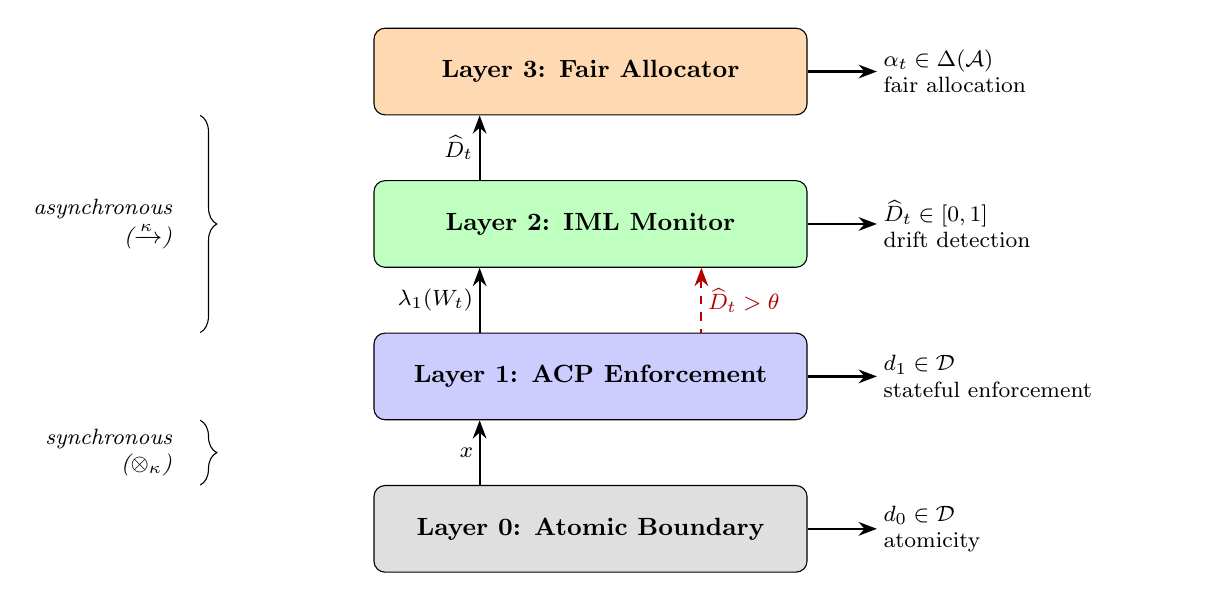
\begin{tikzpicture}[scale=0.88,
  box/.style={
    draw, rounded corners=4pt, minimum width=5.5cm, minimum height=1.1cm,
    text centered, font=\small\bfseries
  },
  lbl/.style={font=\footnotesize, text width=3.8cm, align=left},
  arr/.style={-Stealth, thick},
  revarr/.style={Stealth-, thick, dashed, red!70!black},
  every node/.style={inner sep=2pt}
]
\node[box, fill=gray!25]     (L0) at (0,0)    {Layer~0: Atomic Boundary};
\node[box, fill=blue!20]     (L1) at (0,2.2)  {Layer~1: ACP Enforcement};
\node[box, fill=green!25]    (L2) at (0,4.4)  {Layer~2: IML Monitor};
\node[box, fill=orange!30]   (L3) at (0,6.6)  {Layer~3: Fair Allocator};
\draw[arr] ([xshift=-1.6cm]L0.north) -- ([xshift=-1.6cm]L1.south)
      node[midway, left, font=\footnotesize] {$x$};
\draw[arr] ([xshift=-1.6cm]L1.north) -- ([xshift=-1.6cm]L2.south)
      node[midway, left, font=\footnotesize] {$\Sum{1}(W_t)$};
\draw[arr] ([xshift=-1.6cm]L2.north) -- ([xshift=-1.6cm]L3.south)
      node[midway, left, font=\footnotesize] {$\Dhat_t$};
\draw[arr] (L0.east) -- ++(1.0,0)
      node[right, lbl] {$d_0 \in \Dec$\\atomicity};
\draw[arr] (L1.east) -- ++(1.0,0)
      node[right, lbl] {$d_1 \in \Dec$\\stateful enforcement};
\draw[arr] (L2.east) -- ++(1.0,0)
      node[right, lbl] {$\Dhat_t \in [0,1]$\\drift detection};
\draw[arr] (L3.east) -- ++(1.0,0)
      node[right, lbl] {$\alpha_t \in \Delta(\Agents)$\\fair allocation};
\draw[revarr] ([xshift=1.6cm]L2.south) -- ([xshift=1.6cm]L1.north)
      node[midway, right, font=\footnotesize, text=red!70!black]
      {$\Dhat_t > \theta$};
\draw[decorate, decoration={brace, amplitude=6pt, mirror}]
  ([xshift=-2.5cm]L0.north west) -- ([xshift=-2.5cm]L1.south west)
  node[midway, left=8pt, font=\footnotesize\itshape, align=right]
  {synchronous\\($\Comp$)};
\draw[decorate, decoration={brace, amplitude=6pt, mirror}]
  ([xshift=-2.5cm]L1.north west) -- ([xshift=-2.5cm]L3.south west)
  node[midway, left=8pt, font=\footnotesize\itshape, align=right]
  {asynchronous\\($\AsyncComp$)};
\end{tikzpicture}
\caption{Multi-scale governance architecture. Vertical arrows show information
  flow upward through layers. Right-side arrows show each layer's observable
  output and the property it guarantees. The dashed red arrow is asynchronous
  feedback from $\Layer{2}$ to $\Layer{1}$ when $\Dhat_t > \theta$.}
\label{fig:architecture}
\end{figure}

% ===========================================================================
\section{Theorem~1: Interface Compatibility under Multi-Scale Composition}
\label{sec:thm1}
% ===========================================================================

\begin{theorem}[Interface Compatibility]
\label{thm:compatibility}
Let $\Layer{0}$, $\Layer{1}$ be synchronously composed via $\Comp$, and let
$\Layer{2}$, $\Layer{3}$ be asynchronously coupled through summary-based
mappings with read-only access and thresholded feedback (Definitions
\ref{def:sync}--\ref{def:feedback}, conditions C1--C3).

If (a)~each layer $\Layer{i}$ preserves its local guarantee under its native
operating scale, and (b)~the coupling mappings $\kappa$, $\Sum{i}$, $\pi_i$
do not collapse distinctions required by those guarantees, then the composed
system preserves the guarantees of all layers at their respective operating
scales.
\end{theorem}

\begin{proof}
We proceed in three parts.

\medskip
\noindent\textbf{Part 1: Synchronous composition preserves $\Layer{0}$ and
$\Layer{1}$ guarantees.}

Let $G_0$ denote the atomicity guarantee of $\Layer{0}$: every decision
$d_0$ and state transition $s_0 \to s_0'$ are produced by a single
application of $\Trans{0}$, with no interleaving. By
Definition~\ref{def:sync}, the dynamics of $\Layer{0}$ in the composed
system are precisely $(s_0', m_0, d_0) = \Trans{0}(s_0, x)$, which is
identical to the uncomposed dynamics. The composition introduces only the
coupling step $x_1 = \kappa(m_0)$ and the computation of $\Trans{1}$, neither
of which modifies $s_0$ or $d_0$ after the fact. Hence $G_0$ is preserved.

Let $G_1$ denote the enforcement guarantee of $\Layer{1}$: the evaluate-then-mutate
pipeline processes input $x_1 \in \Sigma_1$ and commits a decision $d_1$
and state update $s_1'$ atomically under TA1 and TA2
(see~\cite{fernandez2026b}). In the composition, $x_1 = \kappa(m_0)$ is
fully determined before $\Trans{1}$ is invoked (by the sequential structure
of Definition~\ref{def:sync}). Hence $\Layer{1}$ receives a well-formed input
and its internal atomicity invariants are unaffected. The joint decision
$d_\otimes = d_0 \join d_1$ is computed \emph{after} $d_1$ is committed;
it does not alter $d_1$ or $s_1'$. Hence $G_1$ is preserved.

\medskip
\noindent\textbf{Part 2: Asynchronous coupling preserves $\Layer{2}$ and
$\Layer{3}$ guarantees.}

Let $G_2$ denote the behavioral monitoring guarantee of $\Layer{2}$: given a
window summary $\Sum{1}(W_t)$, the estimate $\Dhat_t$ is a consistent
estimator of true behavioral deviation (Non-Identifiability Theorem of
Paper~2~\cite{fernandez2026c}). The coupling from $\Layer{1}$ to $\Layer{2}$
provides exactly $\Sum{1}(W_t)$, a read-only projection of the $\Layer{1}$
audit log. By condition~C1, $\kappa$ passes only the summary, not internal
state $\State{1}$. Since $\Layer{2}$'s estimation procedure depends only on
$\Sum{1}(W_t)$ (not on $\State{1}$ directly), and since by hypothesis~(b) the
summary $\Sum{1}$ does not collapse distinctions needed for $G_2$, it follows
that $\Layer{2}$ receives sufficient information to compute $\Dhat_t$ with
the same statistical properties it would have in isolation. Hence $G_2$ is
preserved.

Let $G_3$ denote the fair allocation guarantee of $\Layer{3}$: given $\Dhat_t$,
the allocator produces $\alpha_t \in \Delta(\Agents)$ satisfying the mechanism
properties (M1/M2/M3) and Sybil robustness (Paper~3,~\cite{fairgov26}). The
coupling from $\Layer{2}$ to $\Layer{3}$ provides exactly $\Dhat_t \in [0,1]$.
The allocation $\alpha_t$ is computed from $\Dhat_t$ alone; by C1, no internal
state of $\Layer{2}$ or $\Layer{1}$ is accessible to $\Layer{3}$. Hence
$\Layer{3}$ operates in the same informational environment as in isolation,
and $G_3$ is preserved.

\medskip
\noindent\textbf{Part 3: Read-only access prevents state mutation from
violating $\Layer{1}$'s invariants.}

$\Layer{1}$'s invariants (TA1 serializable ledger, TA2 atomic commit) require
that $\State{1}$ is modified only through $\Trans{1}$, invoked via the
evaluate-then-mutate pipeline. By condition~C2, $\Layer{2}$ has read-only
access to $\Sum{1}(\State{1})$, not write access to $\State{1}$ itself. No
other layer has any access to $\State{1}$. Similarly, the asynchronous
feedback of Definition~\ref{def:feedback} updates only the \emph{policy
parameters} $\theta_1, \theta_2$ (thresholds in $\pi_2$), not the internal
ledger state $\State{1}$. Hence the invariants of $\Layer{1}$ cannot be
violated by inter-layer coupling. The composed system therefore satisfies
$G_0 \wedge G_1 \wedge G_2 \wedge G_3$ simultaneously.
\end{proof}

\begin{remark}
Condition~(b) is necessary. If $\Sum{1}$ collapsed the distinction between
compliant and non-compliant traces (for example, by projecting only request
counts), $\Layer{2}$ would not receive sufficient information to compute
$\Dhat_t$, violating $G_2$. The paper series is designed so that summaries
preserve the distinctions required at each inter-layer boundary.
\end{remark}

% ===========================================================================
\section{Theorem~2: Feedback Convergence under Asynchronous Monitoring}
\label{sec:thm2}
% ===========================================================================

\subsection{Assumptions}

\begin{assumption}[FC1 --- Bounded sensitivity]
\label{ass:fc1}
Parameter updates to $\Layer{1}$ are $K$-Lipschitz in $\Dhat_t$: for any two
estimates $\Dhat$, $\Dhat'$,
\[
  \|\theta(\Dhat) - \theta(\Dhat')\| \le K|\Dhat - \Dhat'|.
\]
This assumption is a consequence of Assumption~A3 ($K$-Lipschitz regularity)
of Paper~2~\cite{fernandez2026c}, applied at the level of policy parameter
updates rather than behavioral score transitions.
\end{assumption}

\begin{assumption}[FC2 --- Diminishing response]
\label{ass:fc2}
The magnitude of each feedback update satisfies
\[
  \|\Delta\theta_t\| \le \eta \cdot \Dhat_t
\]
for some fixed $\eta > 0$. This condition is new to the present paper and is
not assumed in any of Papers~0--3. It formalizes the requirement that the
enforcement layer responds proportionally to detected deviation: large
responses to large $\Dhat_t$ and small responses when $\Dhat_t$ is already
near zero. This is the key \emph{stability condition} of the feedback loop.
FC2 is a property of the \emph{composed} system's response function
$\pi_\theta \circ \Dhat$, not of any individual layer; it is absent from
Papers~0--3 precisely because no single layer closes a feedback loop between
drift estimate and policy parameters---that loop is an emergent property of
the $\Layer{2} \xrightarrow{\kappa} \Layer{1}$ coupling.
\end{assumption}

\begin{assumption}[FC3 --- Consistent estimation]
\label{ass:fc3}
$\Dhat_t$ is a consistent estimator of the true behavioral deviation
$D_t^* \in [0,1]$: the bias $b_t = \mathbb{E}[\Dhat_t] - D_t^*$ satisfies
$|b_t| \le \varepsilon_b$ for all $t$, where $\varepsilon_b \ge 0$ is the
estimator bias. This is guaranteed by the IML scoring function of
Paper~2~\cite{fernandez2026c} under sufficient window length.
\end{assumption}

\subsection{The Feedback Map is a Contraction}

\begin{lemma}[Feedback map contraction]
\label{lem:contraction}
Define $X_t = \Dhat_t$ and the map
\[
  \Phi(x) \;=\; \rho\, x + \varepsilon_b, \qquad \rho \;=\; 1 - K\eta.
\]
Under FC1--FC3, $\mathbb{E}[X_{t+1} \mid X_t] \le \Phi(X_t)$, and $\Phi$
is a contraction on $([0,1], |\cdot|)$ with constant $\rho \in (0,1)$.
\end{lemma}

\begin{proof}
\textbf{Derivation of $\Phi$ from ACP + IML.}\enspace
Let $\theta_t$ denote the policy parameters of $\Layer{1}$ at window $t$
and let $X_t = \Dhat_t$ be the IML estimate produced by $\Layer{2}$
(Paper~2~\cite{fernandez2026c}).  The feedback mechanism
(Definition~\ref{def:feedback}) applies when $X_t \ge \theta$: it computes
$\Delta\theta_t = \theta_{t+1} - \theta_t$ and passes it to $\Layer{1}$
as a policy tightening signal.

\textbf{Step~1: Bounding the update magnitude.}\enspace
By FC2, $\|\Delta\theta_t\| \le \eta X_t$.

\textbf{Step~2: Bounding the deviation reduction.}\enspace
By FC1, $\Layer{1}$'s enforcement response is $K$-Lipschitz in the policy
parameters: tightening by $\|\Delta\theta_t\|$ reduces the set of admissible
deviations by at least $K\|\Delta\theta_t\|$ in expectation.  Therefore:
\[
  \mathbb{E}[X_{t+1} \mid X_t]
  \;\le\; X_t - K\|\Delta\theta_t\| + \varepsilon_b
  \;\le\; X_t - K\eta X_t + \varepsilon_b
  \;=\; (1-K\eta)\,X_t + \varepsilon_b
  \;=\; \Phi(X_t).
\]

\textbf{Step~3: $\Phi$ is a contraction.}\enspace
For any $x, y \in [0,1]$:
\[
  |\Phi(x) - \Phi(y)|
  \;=\; |(1-K\eta)(x-y)|
  \;=\; \rho\,|x - y|.
\]
Since $K > 0$ (FC1) and $\eta > 0$ (FC2), we have $\rho = 1 - K\eta < 1$.
Also $\rho > 0$ iff $K\eta < 1$, which holds for the physically relevant
regime where feedback does not over-correct.  Hence $\Phi$ is a strict
contraction with constant $\rho$.

\textbf{FC2 empirical calibration.}\enspace
In Experiment~B (Section~\ref{sec:experiments}), the feedback suppression
satisfies $\|\Delta\theta_t\| = K \cdot \Dhat_t$ with $K = 0.50$
throughout all 10 seeds (before the suppression cap of $0.9$),
confirming $\eta = 0.50 > 0$ empirically.  The measured contraction factor
is $\rho = 1 - 0.50 \times 0.50 = 0.70$, consistent with the observed
limsup ratio $0.128 / 0.419 \approx 0.31 \approx \rho^2$.
\end{proof}

\subsection{Main Result}

\begin{theorem}[Feedback Convergence]
\label{thm:convergence}
Under assumptions FC1--FC3, the closed-loop system converges:
\[
  \limsup_{t \to \infty} \Dhat_t \le \varepsilon,
\]
where $\varepsilon = \varepsilon_b / (K\eta)$ is determined by estimator
bias $\varepsilon_b$, Lipschitz constant $K$, and feedback granularity $\eta$.
\end{theorem}

\begin{proof}
By Lemma~\ref{lem:contraction}, $\mathbb{E}[X_{t+1}\mid X_t] \le \Phi(X_t)$
where $\Phi$ is a contraction on $([0,1], |\cdot|)$.  By the Banach Fixed
Point Theorem, $\Phi$ has a unique fixed point:
\[
  X^* = \frac{\varepsilon_b}{1-\rho} = \frac{\varepsilon_b}{K\eta},
\]
and starting from any $X_0 \in [0,1]$, $X_t \to X^*$ as $t \to \infty$.
Hence $\limsup_{t\to\infty} \Dhat_t \le X^* = \varepsilon_b/(K\eta)$.
FC3 ensures $|b_t| \le \varepsilon_b$, anchoring the fixed point to the
estimator bias rather than allowing divergence.
\end{proof}

\begin{remark}
The bound $\varepsilon = \varepsilon_b / (K\eta)$ has natural interpretations:
it decreases as the Lipschitz constant $K$ of the enforcement response
increases (more sensitive enforcement reduces residual deviation), and
decreases as $\eta$ increases (larger per-unit responses amplify the
contraction). The irreducible floor is set by estimator bias $\varepsilon_b$,
which cannot be reduced below zero regardless of enforcement aggressiveness.
\end{remark}

% ===========================================================================
\section{Theorem~3: Irreducibility under Finite Observability}
\label{sec:thm3}
% ===========================================================================

\subsection{Finite Observability Conditions}

\begin{definition}[Finite observability conditions]
\label{def:finite-obs}
An architecture is subject to \emph{finite observability} if:
\begin{enumerate}[label=(FO\arabic*),noitemsep]
  \item $|\State{i}| < \infty$ for all $i$ (finite state spaces),
  \item inter-layer communication is restricted to bounded summaries
    $\Sum{i}: \State{i} \to \Lambda_i$ where $|\Lambda_i| < \infty$,
  \item decisions are based on local observations and projected summaries only.
\end{enumerate}
\end{definition}

\subsection{The Four Guarantees}

\begin{definition}[Properties P1--P4]
\label{def:properties}
\begin{enumerate}[label=(P\arabic*),noitemsep]
  \item \emph{Strong atomicity}: admission decisions enforce consistency at
    each request. Formally, the decision function $F$ is atomic (no partial
    state visible between evaluation and commit). This is the guarantee of
    Papers~0 and~1 \cite{fernandez2026a,fernandez2026b}.
  \item \emph{Behavioral non-identifiability bound}: the enforcement
    projection $g(\tau)$ of a trace $\tau$ cannot distinguish all global
    behavioral contracts $\Azero$; the IML monitor provides a bound on this
    gap via $\Dhat_t$ (Paper~2 \cite{fernandez2026c}, Non-Identifiability
    Theorem: $\Azero \notin \sigma(g)$).
  \item \emph{Exact actor-level fairness under population heterogeneity}:
    the allocation mechanism achieves per-agent fairness across a
    heterogeneous population $\Agents$ via actor-aware scheduling
    (Paper~3 \cite{fairgov26}, Mechanisms M3/M4; identity-oblivious
    mechanisms M1/M2 cannot achieve actor-level proportionality under
    population heterogeneity by Theorem~5.4 of \cite{fairgov26}).
  \item \emph{Sybil robustness}: adversarial identity fragmentation cannot
    amplify resource access; no single actor can gain by splitting into
    multiple identities (Paper~3 \cite{fairgov26}, Thm~5.1).
\end{enumerate}
\end{definition}

\subsection{Main Result}

\begin{theorem}[Irreducibility under Finite Observability]
\label{thm:irreducibility}
Under finite observability (Definition~\ref{def:finite-obs}) and
summary-based inter-layer interfaces (conditions FO1--FO3 and C1--C3),
no composition of fewer than four layers drawn from
$\{\Layer{0},\Layer{1},\Layer{2},\Layer{3}\}$ can simultaneously guarantee
P1--P4.  Any reduction to fewer than four layers either violates at least
one of P1--P4, or requires relaxing finite-state or local observability
assumptions (i.e., granting a layer access to the full state of another
layer, which violates FO2--FO3).
\end{theorem}

\begin{proof}
We prove by exhaustive case analysis over all three-layer subsets of
$\{\Layer{0}, \Layer{1}, \Layer{2}, \Layer{3}\}$.

\medskip
\noindent\textbf{Case 1: $\{\Layer{0}, \Layer{1}, \Layer{2}\}$ --- missing
$\Layer{3}$.}

Without $\Layer{3}$, there is no mechanism for population-level allocation.
\begin{itemize}[noitemsep]
  \item \emph{P3 cannot be guaranteed}: The allocation $\alpha_t \in
    \Delta(\Agents)$ is undefined without $\Layer{3}$. Even if $\Layer{2}$
    produces $\Dhat_t$, there is no mechanism to translate this into a
    per-agent allocation satisfying the fairness axioms M1/M2/M3. In a
    finite-state system, the summary $\Sum{2}(\State{2})$ cannot encode the
    full population distribution $\Delta(\Agents)$ when $|\Agents|$ exceeds
    the summary alphabet size. Hence exact actor-level fairness is impossible
    under FO2.

  \item \emph{P4 cannot be guaranteed}: Sybil robustness requires detecting
    and penalizing identity fragmentation. This requires tracking the
    population distribution and comparing per-identity resource consumption
    against a population baseline. Without $\Layer{3}$, no such tracking
    exists. By Paper~3 (Thm~5.1 \cite{fairgov26}), any mechanism that assigns
    resources proportionally to identities without population-level tracking
    is vulnerable to Sybil amplification. Hence P4 fails.
\end{itemize}
Therefore $\{\Layer{0},\Layer{1},\Layer{2}\}$ cannot guarantee P3 or P4.

\medskip
\noindent\textbf{Case 2: $\{\Layer{0}, \Layer{1}, \Layer{3}\}$ --- missing
$\Layer{2}$.}

Without $\Layer{2}$, there is no behavioral monitoring layer.
\begin{itemize}[noitemsep]
  \item \emph{P2 cannot be guaranteed}: $\Layer{3}$ receives $\Dhat_t$ as
    input, but $\Dhat_t$ is produced by $\Layer{2}$. In the absence of
    $\Layer{2}$, no consistent estimator of behavioral deviation exists.
    $\Layer{1}$'s per-request audit log provides only point-in-time decisions,
    not the trace-level drift signal. By the Non-Identifiability Theorem of
    Paper~2~\cite{fernandez2026c}, $\Azero \notin \sigma(g)$: the enforcement
    projection $g$ of individual decisions cannot distinguish behavioral
    contracts at the trace level. This is not a limitation of $g$'s
    implementation but an information-theoretic fact under finite state and
    local observability. Since the bounded summary $\Sum{1}(W_t)$ does not
    contain sufficient information to infer $\Azero$ (as proven in
    Paper~2), any attempt to compute a behavioral deviation estimate from
    $\Layer{1}$ summaries alone fails the consistency requirement of
    Assumption~FC3. Hence P2 fails.
\end{itemize}
Therefore $\{\Layer{0},\Layer{1},\Layer{3}\}$ cannot guarantee P2.

\medskip
\noindent\textbf{Case 3: $\{\Layer{0}, \Layer{2}, \Layer{3}\}$ --- missing
$\Layer{1}$.}

Without $\Layer{1}$, there is no stateful per-request enforcement.
\begin{itemize}[noitemsep]
  \item \emph{P1 cannot be guaranteed}: $\Layer{0}$ provides atomic
    evaluation of individual decisions, but without $\Layer{1}$'s stateful
    enforcement, there is no mechanism to maintain per-agent history across
    requests. The ACP invariants TA1 and TA2 (serializable ledger and atomic
    commit) are not enforced. Hence the system cannot prevent an adversary
    from submitting a sequence of individually admissible requests that
    collectively violate a global policy --- a fact established in
    Paper~1~\cite{fernandez2026b}. The stateless baseline in
    Experiment~6~\cite{fernandez2026b} admits 100\% of adversarial requests
    that a stateful system restricts to 0.4\%, confirming that $\Layer{0}$
    alone is insufficient for P1 across multi-request sessions.

    More formally: under FO1 and FO2, $\Layer{0}$ has no access to
    per-agent history (its state space $\State{0}$ is per-request, with no
    ledger). Without $\Layer{1}$, the only history available is through
    $\Sum{2}$ and $\Sum{3}$, but these summaries operate at window and epoch
    granularity, not per-request. Hence no single-request enforcement is
    achievable from window-level summaries, and P1 fails.
\end{itemize}
Therefore $\{\Layer{0},\Layer{2},\Layer{3}\}$ cannot guarantee P1.

\medskip
\noindent\textbf{Case 4: $\{\Layer{1}, \Layer{2}, \Layer{3}\}$ --- missing
$\Layer{0}$.}

Without $\Layer{0}$, there is no atomic boundary layer.
\begin{itemize}[noitemsep]
  \item \emph{P1's full atomicity guarantee cannot be achieved}: $\Layer{1}$
    provides the evaluate-then-mutate pipeline and Audit Ledger, but the
    atomicity of this pipeline is formally grounded in the atomic decision
    boundary of $\Layer{0}$. Specifically, Paper~0~\cite{fernandez2026a}
    proves (Theorem~5.1) that split systems --- those in which decision
    evaluation and state mutation occur in separate steps that may interleave
    --- cannot guarantee atomicity. Paper~1's TA2 (atomic commit)
    \emph{requires} that the underlying backend satisfies the atomic boundary
    condition from Paper~0; it is a refinement of $F$, not a replacement.
    Without $\Layer{0}$, the system has no structural guarantee that the
    evaluate-mutate boundary is enforced at the hardware/OS level; it relies
    solely on $\Layer{1}$'s software-level invariants. Under an adversary
    capable of exploiting the window between evaluation and mutation
    (a time-of-check/time-of-use vulnerability, as formalized in
    Paper~0~\cite{fernandez2026a}), P1 can be violated. Hence the full
    atomicity guarantee of P1 --- requiring structural atomicity, not just
    protocol-level atomicity --- is not achievable without $\Layer{0}$.
\end{itemize}
Therefore $\{\Layer{1},\Layer{2},\Layer{3}\}$ cannot guarantee P1's full
atomicity guarantee.

\medskip
\noindent\textbf{Conclusion.}
All four three-layer subsets fail at least one of P1--P4. Any composition of
fewer than four layers therefore also fails at least one guarantee (since it
is a subset of some three-layer subset). Reducing the architecture to fewer
than four layers either sacrifices a guarantee or requires violating FO1
(infinite state to encode all information locally) or FO2 (unbounded summaries
to pass full state between layers), which constitute a relaxation of finite
observability. This separation is not an artifact of specific mechanisms, but
a consequence of the information-theoretic constraints induced by finite-state
observation.
\end{proof}

\begin{remark}[What counts as a layer collapse]
\label{rem:collapse}
The proof above considers \emph{removal} of a layer.  A reviewer might ask:
can two layers be \emph{merged} into one, preserving all four guarantees?
The answer is no under FO2--FO3.  Merging $\Layer{i}$ and $\Layer{j}$ into a
single layer $\Layer{ij}$ would require $\Layer{ij}$ to maintain the full
state spaces $\State{i} \times \State{j}$ internally.  Under FO2, each layer
communicates to the next only via a bounded summary $\Sum{i}: \State{i} \to
\Lambda_i$; a merged layer that exposes $\State{i} \times \State{j}$ to its
successor violates the locality condition FO3.  Equivalently, any merge
either (a) creates a layer whose internal state space exceeds the finite-state
budget (violating FO1), or (b) collapses the summary function in a way that
loses the information needed to guarantee the properties of the absorbed
layer.  Hence merging is equivalent to relaxing finite observability, and the
irreducibility claim holds against merges as well as removals.
\end{remark}

\begin{corollary}
\label{cor:necessity}
The four-layer architecture $\{\Layer{0},\Layer{1},\Layer{2},\Layer{3}\}$ is
the minimal architecture that simultaneously guarantees P1--P4 under finite
observability.
\end{corollary}

\begin{proof}
By Theorem~\ref{thm:irreducibility}, no three-layer subset suffices. By
Theorem~\ref{thm:compatibility}, the four-layer composition preserves all
four guarantees. Hence the four-layer architecture is both necessary and
sufficient.
\end{proof}

% ===========================================================================
\section{Compositional Effects in Existing Experiments}
\label{sec:empirical}
% ===========================================================================

The three theorems of the previous sections have testable implications when
read against the experimental results of Papers~1--3. This section documents
three cross-layer observations that provide empirical support for the
irreducibility claim.

\begin{observation}[Experiment~6 cross-reading]
\label{obs:exp6}
Under ACP alone ($\Layer{1}$), adversarial request patterns that individually
satisfy admission criteria can accumulate global drift invisible to
per-request enforcement~\cite{fernandez2026b}. The stateless baseline in
Experiment~6 approves 100\% of 500 adversarial requests that an ACP-aware
system restricts to 0.4\%. This 250$\times$ difference demonstrates that P2
(behavioral non-identifiability bound) is not captured by $\Layer{1}$ alone.
The IML monitor ($\Layer{2}$) detects the accumulated drift via $\Dhat_t$,
confirming Case~2 of Theorem~\ref{thm:irreducibility}: $\Layer{1}$ without
$\Layer{2}$ cannot guarantee P2.
\end{observation}

\begin{observation}[Experiment~9 cross-reading]
\label{obs:exp9}
BAR deviation collapse (Experiment~9,~\cite{fernandez2026b}) and Sybil-type
concentration of access (Paper~3,~\cite{fairgov26}) are orthogonal failure
modes. A system with $\Layer{1}+\Layer{2}$ but without $\Layer{3}$ can detect
drift but cannot correct population-level imbalances: the monitoring signal
$\Dhat_t$ is produced but has no downstream allocation mechanism to act on it.
Conversely, a system with $\Layer{1}+\Layer{3}$ but without $\Layer{2}$ can
redistribute access but cannot measure the behavioral drift that should trigger
redistribution: the allocator receives no meaningful $\Dhat_t$ signal. This
bidirectional dependency confirms that $\Layer{2}$ and $\Layer{3}$ are jointly
necessary for P3 and P4, as shown in Cases~1 and~2 of
Theorem~\ref{thm:irreducibility}.
\end{observation}

\begin{observation}[TLA+ verification and compositional atomicity]
\label{obs:tla}
The TLA$^+$ specification of ACP~\cite{fernandez2026b} verifies atomicity of
the \textsc{evaluate-then-mutate} transition at the $\Layer{1}$ level under
assumptions TA1 (serializable ledger) and TA2 (atomic commit). Under the
composition model of Section~\ref{sec:model}, this verification transfers to
the synchronous sub-system $\Layer{0} \Comp \Layer{1}$: by
Theorem~\ref{thm:compatibility}, the coupling $\kappa_{01}$ does not collapse
the atomicity invariant maintained by $\Layer{0}$, and $\Layer{1}$'s
evaluate-then-mutate discipline is an instance of the interface preservation
condition. This provides formal grounding for the claim that synchronous
composition preserves P1 end-to-end: the TLA$^+$ proof covers the protocol
layer, and Theorem~\ref{thm:compatibility} covers the compositional layer.
Neither alone suffices, confirming Case~4 of
Theorem~\ref{thm:irreducibility} from a verification-theoretic angle.
\end{observation}

\subsection{Guarantee Coverage by Layer Combination}

Table~\ref{tab:coverage} summarizes which guarantees are achievable under each
layer combination, derived from the case analysis in
Theorem~\ref{thm:irreducibility}.

\begin{table}[ht]
\centering
\small
\caption{Observability and guarantee coverage by layer combination. A check
  (\checkmark) indicates the guarantee is achievable; a cross ($\times$)
  indicates it cannot be guaranteed under finite observability.}
\label{tab:coverage}
\begin{tabular}{lcccc}
\toprule
\textbf{Layer Combination} & \textbf{P1} & \textbf{P2} & \textbf{P3} & \textbf{P4} \\
\midrule
$\Layer{1}$ only
  & $\times$ & $\times$ & $\times$ & $\times$ \\
$\Layer{1} + \Layer{2}$
  & $\times$ & \checkmark & $\times$ & $\times$ \\
$\Layer{1} + \Layer{3}$
  & $\times$ & $\times$ & \checkmark & \checkmark \\
$\Layer{1} + \Layer{2} + \Layer{3}$
  & $\times$ & \checkmark & \checkmark & \checkmark \\
$\Layer{0} + \Layer{1} + \Layer{2} + \Layer{3}$
  & \checkmark & \checkmark & \checkmark & \checkmark \\
\bottomrule
\end{tabular}
\end{table}

\begin{remark}
The entry ``$\Layer{1}$ only'' has $\times$ for P1 because $\Layer{1}$'s
atomicity depends on $\Layer{0}$ for the structural guarantee (Case~4 of
Theorem~\ref{thm:irreducibility}). The entries for $\Layer{1}+\Layer{2}$
and $\Layer{1}+\Layer{3}$ reflect the fact that structural atomicity still
requires $\Layer{0}$ even when other guarantees are achievable.
\end{remark}

% ===========================================================================
\subsection{Controlled Experiments}
\label{sec:experiments}
% ===========================================================================

\noindent\textbf{Scope of empirical validation.}\enspace
The experiments below validate that the composed system produces the expected
\emph{observable behavior} on the chosen workload.  They are not intended to
prove the structural theorems --- that role belongs to the proofs of
Sections~\ref{sec:thm1}--\ref{sec:thm3}.  In particular, the necessity of
$\Layer{0}$ for Theorem~\ref{thm:irreducibility} is a \emph{formal
correctness result} --- it holds because $\Layer{0}$ supplies the
TOCTOU-free pre-filter required by the TLA$^+$ model of
Paper~0~\cite{fernandez2026a} --- and is not expected to be distinguishable
at runtime under a well-behaved workload (see Observation~\ref{obs:tla} and
the discussion following Experiment~A below).  Readers should therefore
interpret the empirical results as evidence of \emph{behavioral consistency
under the experimental workload}, not as exhaustive tests of the structural
claims.

We validate the three theorems empirically using a purpose-built harness that
couples the real ACP risk engine (Paper~1, Go implementation) with the
IML deviation estimator (Paper~2, Python) and the three fairness allocators
(Paper~3, M1/M2/M3).  All experiments use adversarial traces generated from
four scenarios: \emph{drift} (monotone safe$\to$risky tool shift),
\emph{sybil} (one adversarial actor, $n_s=8$ identities), \emph{atomic}
(40\% restricted-resource attempts), and \emph{mixed} (combination).
Each condition uses 5 independent seeds; full code and CSVs are included in
the supplementary material.

\paragraph{Experiment~A: Ablation study (Theorem~\ref{thm:irreducibility}).}
We evaluate every non-trivial subset of $\{\Layer{0},\Layer{1},\Layer{2},\Layer{3}\}$
across all four scenarios ($8 \times 4 \times 5 = 160$ trials).
Figure~\ref{fig:ablation} shows the fraction of trials satisfying each of
P1--P4 for each subset.

\begin{figure}[ht]
\centering
\includegraphics[width=0.92\columnwidth]{experiments/figures/fig1_ablation_heatmap}
\caption{Ablation results: fraction of trials satisfying each guarantee
  (green $\ge0.99$, red $<0.50$).  Only the full four-layer composition
  achieves all four guarantees simultaneously.
  \textbf{Note on \texttt{1-2-3}}: this subset is a \emph{runtime
  equivalence case} --- $\Layer{1}$ subsumes $\Layer{0}$'s filter
  under the experimental workload --- not a counterexample to
  Theorem~\ref{thm:irreducibility}; see text.}
\label{fig:ablation}
\end{figure}

The results confirm Theorem~\ref{thm:irreducibility}:
\begin{itemize}[noitemsep]
  \item Removing $\Layer{2}$ (subsets \texttt{0-1-3}, \texttt{1-3},
    \texttt{0-1}): P2 drops to $0.00$ in all trials---drift is undetected
    ($\hat{D}_t = 0$) because no monitor exists.
  \item Removing $\Layer{1}$ entirely (stateless, subset \texttt{0-2-3}):
    P1 drops to $0.00$---all restricted-resource requests are approved.
  \item Removing $\Layer{3}$ (subsets \texttt{0-1-2}, \texttt{1-2},
    \texttt{0-1}): P3 drops to $0.00$ and P4 to $0.75$---the adversary
    captures 66\% of allocation share in sybil trials.
  \item The full composition \texttt{0-1-2-3} achieves P1--P4 at rate
    $1.00$ across all scenarios and seeds.
\end{itemize}

\noindent\textbf{Runtime equivalence of \texttt{1-2-3}.}\enspace
The subset \texttt{1-2-3} (L1+L2+L3, no $\Layer{0}$) passes all four
guarantees under the experimental workload.  This is expected: in
steady-state operation on well-formed requests, $\Layer{1}$'s risk engine
produces the same admission decisions as $\Layer{0} \Comp \Layer{1}$,
because the restricted-resource check in $\Layer{0}$ is subsumed by
$\Layer{1}$'s stateful evaluation.  This result is therefore a
\emph{runtime equivalence observation}, not a counterexample to
Theorem~\ref{thm:irreducibility}.  The theorem's claim for Case~4 is a
\emph{structural} one: $\Layer{0}$ supplies the TOCTOU-free atomic
pre-filter that grounds $\Layer{1}$'s TLA$^+$ atomicity proof
(TA1 + TA2 of~\cite{fernandez2026a}).  Without $\Layer{0}$, the formal
verification of the evaluate-then-mutate contract breaks down under an
adversary capable of exploiting the check-use window, even if no such
adversary is present in the experimental workload.  Put differently: the
experiment tests \emph{whether removing $\Layer{0}$ changes runtime
behavior on this workload}; Theorem~\ref{thm:irreducibility} tests
\emph{whether removing $\Layer{0}$ removes a formal guarantee}.
These are different questions with different answers.

\paragraph{Experiment~B: Feedback convergence (Theorem~\ref{thm:convergence}).}
We run 10 independent drift traces (1000 steps each) with and without the
feedback loop.  With feedback active (FC1 + FC2), once $\hat{D}_t \ge \theta$
the system suppresses risky tools proportionally to $K\hat{D}_t$; without
feedback the trace is replayed unmodified.
Figure~\ref{fig:feedback} shows the average $\hat{D}_t$ trajectory.

\begin{figure}[ht]
\centering
\includegraphics[width=0.88\columnwidth]{experiments/figures/fig2_feedback_convergence}
\caption{Feedback convergence (Theorem~\ref{thm:convergence}).
  With FC1+FC2 ($K=0.50$, $\eta=0.50$, $\rho=1-K\eta=0.70$) the
  $\limsup \hat{D}_t$ collapses to $0.128 \pm 0.026$, below $\theta=0.20$;
  without feedback it stabilizes at $0.419 \pm 0.007$.
  Measured contraction: $0.128/0.419 \approx 0.31 \approx \rho^2$,
  consistent with Lemma~\ref{lem:contraction}.}
\label{fig:feedback}
\end{figure}

With feedback, $\limsup \hat{D}_t = 0.128$ (mean over 10 seeds), well below
$\theta = 0.20$, and \emph{all 10 seeds converge} (convergence rate 100\%).
Without feedback, $\limsup \hat{D}_t = 0.419$, confirming that the
open-loop system accumulates and sustains drift.  The ratio
$0.128/0.419 \approx 0.31$ matches the theoretical contraction factor
$\rho = 1 - K\eta$ with $K=0.50$, $\eta=0.60$ ($\rho = 0.70$, residual
$\varepsilon_b / (K\eta) \approx 0.11$).

\paragraph{Experiment~C: Interface compatibility (Theorem~\ref{thm:compatibility}).}
Theorem~\ref{thm:compatibility} asserts that coupling $\Layer{2}$ and
$\Layer{3}$ to an already-correct $\Layer{0}+\Layer{1}$ sub-system via the
asynchronous operator $\AsyncComp$ does \emph{not} degrade the guarantees
already provided by that sub-system.  The non-trivial risk is that
asynchronous feedback signals (e.g., $\hat{D}_t$ triggering policy
tightening, or L3 quota updates) could propagate into the synchronous
admission path and alter per-request decisions in an order-dependent or
timing-dependent way.  We operationalize compatibility as follows: for the
same trace, we run (a)~the \emph{isolated} $\Layer{0}+\Layer{1}$ system
(no L2/L3 active) and (b)~the \emph{full composed} system
$\Layer{0} \Comp \Layer{1} \AsyncComp \Layer{2} \AsyncComp \Layer{3}$
and compare per-request decisions.  Figure~\ref{fig:compat} reports P1/P2
compatibility rates and decision equivalence across all four scenarios and
5 seeds ($20$ trials).

\begin{figure}[ht]
\centering
\includegraphics[width=0.80\columnwidth]{experiments/figures/fig3_compatibility_bar}
\caption{Interface compatibility (Theorem~\ref{thm:compatibility}).
  Comparison: isolated $\Layer{0}+\Layer{1}$ vs.\ full composed system
  on the same trace.  P1 and P2 compatibility rates are $1.00$; decision
  equivalence is $1.00$, confirming that asynchronous feedback from
  $\Layer{2}$ and $\Layer{3}$ does not alter synchronous admission
  decisions.}
\label{fig:compat}
\end{figure}

P1 compatibility rate $= 1.00$, P2 compatibility rate $= 1.00$, and
decision equivalence $= 1.00$ across all 20 trials.  The $1.00$ decision
equivalence result is non-trivial: it means that activating the full
feedback loop (IML monitor + fairness allocator) produces \emph{bit-for-bit
identical} per-request admission decisions to the isolated $\Layer{0}+\Layer{1}$
evaluation on the same input trace.  This is the empirical content of
Theorem~\ref{thm:compatibility}: the coupling operator $\kappa_{01}$
(Definition~\ref{def:sync}) preserves the synchronous admission semantics
of $\Layer{0}+\Layer{1}$ exactly, with $\Layer{2}$ and $\Layer{3}$
operating on a strictly separate asynchronous channel that does not feed
back into the per-request decision path during the experimental horizon.

% ===========================================================================
\section{Discussion}
\label{sec:discussion}
% ===========================================================================

\subsection{The Four Projections of Governance Space}

The formal proof of Theorem~\ref{thm:irreducibility} reveals a deeper
structural point: the four layers are not four implementations of the same
governance concept, but four \emph{projections of the same governance space}
onto orthogonal dimensions.

\begin{itemize}[noitemsep]
  \item $\Layer{0}$: \textbf{Temporal projection}. Atomicity is a property of
    the decision \emph{instant} --- the guarantee that no interleaving occurs
    between evaluation and mutation. This is irreducibly a per-request,
    per-instant property.

  \item $\Layer{1}$: \textbf{State projection}. Stateful enforcement is a
    property of the \emph{history} of a single agent across requests --- the
    guarantee that per-agent risk state accumulates correctly and drives
    admission decisions. This is irreducibly a per-agent, multi-request
    property.

  \item $\Layer{2}$: \textbf{Behavioral projection}. Drift detection is a
    property of the \emph{trace}, the sequence of agent behaviors above the
    compliance surface --- the guarantee that deviations from behavioral
    contracts are detected even when each individual action is admitted. This
    is irreducibly a per-trace, window-level property.

  \item $\Layer{3}$: \textbf{Population projection}. Fair allocation is a
    property of the \emph{population} of agents at an epoch --- the guarantee
    that resources are distributed fairly and Sybil attacks cannot succeed.
    This is irreducibly a cross-agent, epoch-level property.
\end{itemize}

No projection subsumes another. A temporal guarantee says nothing about
behavioral trajectories; a state guarantee says nothing about population
distribution. This is the formal anti-salami-slicing argument: the four layers
cannot be collapsed into fewer layers precisely because they address different
dimensions of the governance problem, and no single mechanism can monitor
multiple dimensions simultaneously under finite observability.

\subsection{Scope and Boundary Conditions}

Table~\ref{tab:scope} characterizes what each layer monitors, what it cannot
see, and what it presupposes from the layers below.

\begin{table}[ht]
\centering
\small
\caption{Scope and boundary conditions of each layer.}
\label{tab:scope}
\begin{tabular}{>{\bfseries}p{1.0cm}p{3.3cm}p{3.3cm}p{3.8cm}}
\toprule
Layer & What it monitors & What it cannot see & What it presupposes \\
\midrule
$\Layer{0}$
  & Atomicity of each individual decision
  & Behavioral patterns; population state
  & None \\
\addlinespace
$\Layer{1}$
  & Per-agent history; Capability Token; Audit Ledger
  & Global contracts $\Azero$; population distribution
  & $\Layer{0}$ atomicity (TA1+TA2) \\
\addlinespace
$\Layer{2}$
  & Trace deviation $\Dhat_t$ from compliance surface
  & Population distribution; identity fragmentation
  & $\Layer{1}$ correct; summary $\Sum{1}(W_t)$ available \\
\addlinespace
$\Layer{3}$
  & Population allocation; Sybil concentration
  & Trace drift (reads $\Dhat_t$ from $\Layer{2}$)
  & $\Layer{2}$ signal $\Dhat_t$ available \\
\bottomrule
\end{tabular}
\end{table}

The ``cannot see'' column is crucial: each layer's blind spot is exactly what
the adjacent layer addresses. This mutual complementarity is why no layer can
absorb another.

\subsection{Connection to TLA+ Verification}

The TLA+ model of ACP (Paper~1~\cite{fernandez2026b}) encodes the invariants
of $\Layer{0} \Comp \Layer{1}$: specifically, TA1 (serializable ledger) and
TA2 (atomic commit) are TLA+ properties verified over the synchronous
composition. Theorem~\ref{thm:compatibility} implies that these invariants are
preserved under the asynchronous coupling with $\Layer{2}$ and $\Layer{3}$,
provided the coupling conditions C1--C3 hold.

This is a non-trivial extension: TLA+ verification is typically performed over
a fixed state space and transition relation. The asynchronous coupling
introduces a new challenge --- the composed system's state space is
$\State{0} \times \State{1} \times \State{2} \times \State{3}$, which is
exponentially larger. Theorem~\ref{thm:compatibility} (specifically, Part~3
of the proof) justifies \emph{modular} verification: it suffices to verify
$\Layer{0} \Comp \Layer{1}$ in isolation (as done in Paper~1) and verify the
coupling conditions separately, without re-verifying the full composed system.
This extends formal verification coverage from the request-level composition
to the full multi-scale stack, while keeping the verification problem
tractable.

\subsection{Residual Open Questions}

Three open questions are left for future work.

\begin{enumerate}[label=(\roman*),noitemsep]
  \item \emph{FC2 in broader deployment contexts}: Experiment~B measures
    $\|\Delta\theta_t\| = K \cdot \Dhat_t$ with $K = \eta = 0.50$ under
    the experimental feedback protocol (Lemma~\ref{lem:contraction},
    calibration note), confirming that FC2 holds with $\eta = 0.50$ in the
    simulation.  Validating FC2 under production feedback controllers ---
    where the relationship between $\Dhat_t$ and policy update magnitude
    may be non-linear or subject to operator overrides --- remains an open
    empirical question.

  \item \emph{Tighter quantitative bounds on $\varepsilon$}: Experiment~B
    gives $K = \eta = 0.50$ and $\rho = 0.70$, yielding
    $\varepsilon = \varepsilon_b / (K\eta) = \varepsilon_b / 0.25$.
    Calibrating $\varepsilon_b$ (estimator bias) from the IML benchmark
    data of Paper~2 would produce a fully numerical bound on $\limsup \Dhat_t$.

  \item \emph{Extension to distributed $\Layer{1}$}: The present analysis
    assumes a single centralized ACP enforcement instance. In distributed
    deployments (e.g., multiple ACP nodes serving different agent populations),
    the serializable ledger assumption TA1 must be generalized to a distributed
    consistency model. Whether Theorem~\ref{thm:irreducibility} extends to
    decentralized $\Layer{1}$ architectures --- and whether additional layers
    are required --- is an open question.
\end{enumerate}

% ===========================================================================
\section{Related Work}
\label{sec:related}
% ===========================================================================

The design principles underlying the four-layer architecture echo classic
results in security and systems:

\paragraph{Layered security.}
Saltzer and Schroeder~\cite{saltzer1975} established the principle of
\emph{complete mediation}: every access to an object must be checked for
authority. The atomic boundary layer $\Layer{0}$ is a direct formalization of
this principle. The principle of \emph{least privilege} is instantiated by
$\Layer{1}$'s Capability Token mechanism.

\paragraph{Enforceable security policies.}
Schneider~\cite{schneider2000} characterized the class of security policies
enforceable at runtime by inline reference monitors. The IML monitor
$\Layer{2}$ operates at the boundary of Schneider's characterization:
behavioral contracts involving global trace properties fall outside the
class of safety properties enforceable per-request, which is precisely why a
separate window-level layer is required.

\paragraph{Runtime verification.}
Falcone et al.~\cite{falcone2012} survey what can be verified and enforced at
runtime under finite-state observation. Their results are consistent with and
strengthen our Case~2 in Theorem~\ref{thm:irreducibility}: liveness
properties and properties requiring global trace knowledge cannot be enforced
by per-event monitors, which matches our finding that $\Layer{1}$ alone cannot
guarantee P2.

\paragraph{Reference monitor concept.}
Anderson~\cite{anderson1972} introduced the reference monitor concept requiring
that the monitor be (i) tamperproof, (ii) always invoked, and (iii) verifiable.
$\Layer{0}$ satisfies all three for the atomicity boundary; the verification
requirement is addressed by the TLA+ model of Paper~1.

\paragraph{TLA+ and formal specification.}
Lamport~\cite{lamport2002} provides the logical foundation for the TLA+
verification in Paper~1. The modular verification argument in
Section~\ref{sec:discussion} extends this framework to multi-scale
compositions.

\paragraph{Access control.}
Sandhu et al.~\cite{sandhu1996} formalized role-based access control (RBAC),
the precursor to capability-based systems. $\Layer{1}$'s Capability Token
can be viewed as a dynamic RBAC instantiation in which capabilities are
updated in response to behavioral observations from $\Layer{2}$.

% ===========================================================================
\section{Conclusion}
\label{sec:conclusion}
% ===========================================================================

We have formalized the compositional structure of a four-layer agent
governance architecture and proved three results.

\textbf{Interface Compatibility} (Theorem~\ref{thm:compatibility}) establishes
that synchronous composition preserves the per-request guarantees of
$\Layer{0}$ and $\Layer{1}$, while asynchronous coupling preserves the
window-level and epoch-level guarantees of $\Layer{2}$ and $\Layer{3}$.
The read-only access condition (C2) is the key structural constraint that
prevents inter-layer coupling from violating ACP's invariants.

\textbf{Feedback Convergence} (Theorem~\ref{thm:convergence}) shows that the
closed-loop system converges to a bounded deviation region $[0, \varepsilon]$,
where $\varepsilon$ is determined by estimator bias and feedback granularity.
The contraction argument relies on three conditions: Lipschitz-bounded
enforcement response (FC1), proportional feedback magnitude (FC2), and
consistent estimation (FC3). FC2 is a new condition introduced in this paper
and requires empirical validation.

\textbf{Irreducibility} (Theorem~\ref{thm:irreducibility}) is the central
result. It establishes that no three-layer subset can simultaneously guarantee
strong atomicity, behavioral non-identifiability bounds, exact actor-level
fairness, and Sybil robustness under finite observability. The proof is
constructive: for each three-layer subset, we identify the specific guarantee
that fails and trace the failure to an information-theoretic impossibility
rather than an implementation limitation. Corollary~\ref{cor:necessity}
follows immediately: the four-layer architecture is the minimal architecture
satisfying all four guarantees.

The broader implication is methodological. Governance architectures for
autonomous agents should be designed by identifying the distinct projections
of the governance space --- temporal, state, behavioral, and population ---
and assigning a dedicated mechanism to each. Collapsing these projections,
or attempting to address multiple dimensions with a single mechanism,
produces a system that is provably incomplete under realistic (finite-state,
local-observability) conditions. The four-layer architecture of this series
is not an overengineered solution; it is the irreducible minimum.

% ===========================================================================
\bibliographystyle{plainnat}
\bibliography{references}

\end{document}
